%!TEX root=./paper.tex
\section{System Model}\label{sec:system-model}
\subsection{\textbf{Data streaming framework}}

Reliable real-time data collection is a crucial aspect and prerequisite of a digital twin to effectively update internal parameters and synchronize with the real world. The Traffic Digital Twin, \name, presented in this paper, requires real-time traffic volume data as input. We aim to use absolute traffic volume counts available at a manageable low frequency of 15 minutes to one hour. While systems with more sophisticated data at a higher frequency can be proposed, our goal is to maintain the collection infrastructure as affordable, straightforward, and compatible with already existing systems globally. 

Our proposed system aims to ensure practicality and adaptability as follows. First, the hardware infrastructure should be inexpensive and easily replaceable. Second, the system should be easily extendable to incorporate various data sources. Third, it should function effectively using only absolute traffic counts, without requiring additional specific information such as direction and vehicle types. Finally, the system should operate with a medium-frequency update.

% \begin{enumerate}[(i)]
%     \item Hardware infrastructure should be cheap and easily replaceable.
%     \item Easily extendable to use a variety of different sources.
%     \item Should work with only absolute traffic counts, no other specific information like direction and vehicle types.
%     \item Should work with a medium-frequency update.
% \end{enumerate}

\begin{figure*}
  \centering
  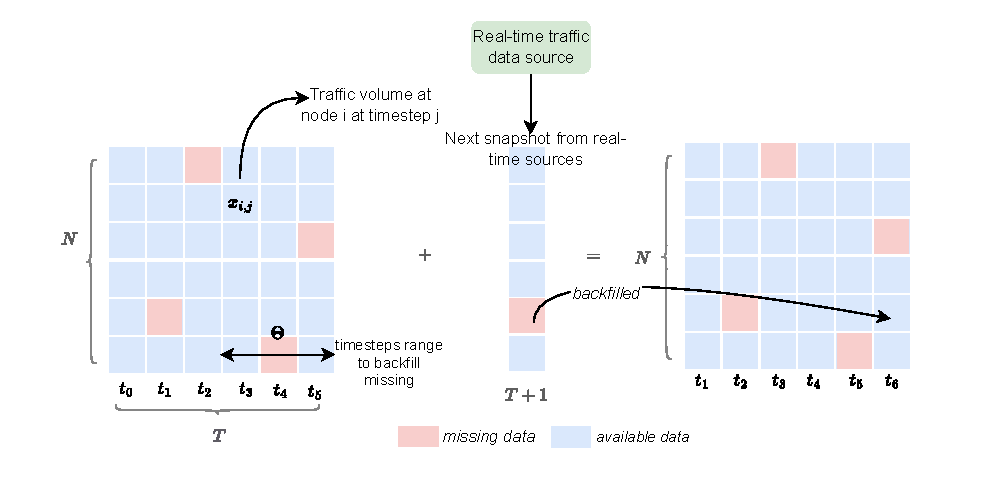
\includegraphics[width=0.85\textwidth]{backfill_fig.pdf}
  \caption{\name \ Merging real-time traffic data from sensors with existing data to get a window of T timesteps}
  \label{fig:backfill}
\end{figure*}

Various methods can be employed to collect the necessary data. The most reliable method involves installing inductive loop detectors embedded in road surfaces at city intersections. These systems are already operational in several major cities. For instance, the Sydney Coordinated Adaptive Traffic System (SCATS)~\cite{scats} is utilized in over 180 cities across 28 countries, including New Zealand, Dublin, Shanghai, and Hong Kong~\cite{wiki:sydney_traffic_system}. Other examples include New York City's Adaptive Traffic Control System (ATCS), Adaptive Signal Control Technology (ASCT), SCOOT, and ACS, which are designed to control traffic signal timings and mitigate congestion. These systems can be seamlessly integrated with our proposed model, as they are capable of collecting the absolute traffic volume counts required for our analysis.

Another potential data source involves the use of surveillance cameras combined with computer vision models \cite{jain2019review}, which are already implemented at certain intersections in Shenzhen, China. Several existing studies \cite{asha2018vehicle} employing state-of-the-art object detection models, such as YOLO \cite{redmon2018yolov3}, have demonstrated the effectiveness of this method. This model-based approach enables cost-effective and efficient traffic monitoring utilizing the existing surveillance camera infrastructure.


Other methods, such as using GPS-enabled mobile phones \cite{rose2006mobile} to track urban traffic flow, as implemented by Google in its Maps product, and the use of probe vehicles \cite{zhu2012probe}, which are vehicles equipped with detectors that may be taxis or public transport, can also be utilized to approximate traffic volume based on their data.

We aim for our model to work in conjunction with multiple data streams, as different parts of the road network may be served with different data sources. We want our \name to integrate with these sources seamlessly, so we need an aggregator to reconcile the data from the different streams and store them in a data lake. This data can then be used by \name to keep its internal state in sync with real-world data.

One way to deploy the aggregator system is to equip it with both RPC and API interfaces for interaction with remote sensors and various data sources. Each service can integrate a separate interface specifically designed to interface with the aggregator. Subsequently, the aggregator consolidates all incoming data, along with relevant meta information, into a datalake—a centralized repository capable of handling both structured and unstructured data. This approach leverages the datalake's capacity to store additional information beyond traffic volume counts from diverse sources, paving the way for potential future enhancements and expansions of \name's capabilities.

A simplified representation of the aforementioned process is depicted in Fig. \ref{fig:framework}.

\subsection{\textbf{Syncing with realtime data and re-learning}}

As a Digital Twin, there's two problems we must address, which are as following:

\subsubsection{Syncing Internal State with Realtime Data}\label{subsubsec:sync}

The Digital Twin synchronization mechanism incorporates a robust state update strategy that dynamically integrates real-time measurements while maintaining system state continuity.

Let $\mathbf{S}_t = [s_{1,t}, s_{2,t}, \ldots, s_{n,t}]$ represent the system state vector at time $t$, where each $s_{i,t}$ corresponds to a specific traffic parameter such as volume, speed, or occupancy for different road segments.

The state update is governed by the equation:

\begin{equation}\label{eq:state_update}
\mathbf{S}_{t+\Delta t} = \mathbf{D}_{\text{real}} \odot \mathbf{M} + \mathbf{S}_t \odot (1 - \mathbf{M}) \odot \mathbf{\Theta}
\end{equation}

\textbf{Mask Definitions:}

The mask $\mathbf{M}$ is defined as a vector of binary indicators for data presence:

\begin{equation}
\mathbf{M} = \begin{cases} 
1 & \text{if } \mathbf{D}_{\text{real}} \text{ is available} \\
0 & \text{otherwise}
\end{cases}
\end{equation}

The threshold matrix $\mathbf{\Theta}$ is defined based on the temporal difference between current and previous measurements:

\begin{equation}
\mathbf{\Theta} = \begin{cases} 
1 & \text{if } |t_{\text{current}} - t_{\text{previous}} | \leq T_{\text{threshold}} \\
0 & \text{otherwise}
\end{cases}
\end{equation}

Where:
\begin{itemize}
    \item $t_{\text{current}}$ is the timestep of the current measurement
    \item $t_{\text{previous}}$ is the timestep of the previous measurement in state
    \item $T_{\text{threshold}}$ is a predefined timestep threshold
\end{itemize}

The key idea being selecting latest data and falling back to older data if it's not available, while still maintaining that we do not use data that is too stale. This approach enables adaptive synchronization, handling sparse and heterogeneous data streams while preserving the Digital Twin's state integrity by selectively incorporating measurements based on both data availability and temporal consistency. An illustrative example can be seen in Fig. \ref{fig:backfill}

\subsubsection{Re-learning based on updated traffic dynamics}\label{subsubsec:sync}

To maintain the accuracy and reliability of the Digital Twin, continuous learning from updated traffic dynamics is essential. Traffic patterns evolve due to various factors such as infrastructure changes, policy updates, and seasonal variations. Therefore, it is necessary to adapt the system periodically through a re-learning process.

Given the inherently noisy nature of real-time traffic data, performing continuous re-training at short intervals may introduce significant volatility and reduce predictive stability. To mitigate this, we propose a periodic re-learning strategy, executed at fixed intervals, such as on a weekly basis. This approach balances responsiveness to new traffic conditions while minimizing noise-induced instability.

A sliding window mechanism can be used for re-learning, where the training dataset continuously evolves by discarding the oldest data and appending the most recent observations. This method ensures that the model remains updated with recent traffic patterns while retaining historical context for better generalization.

Importantly, the re-learning process does not involve training the model from scratch. Instead, the model undergoes fine-tuning using newly available data, leveraging pre-existing knowledge to accelerate adaptation while preserving stability.

Let $\mathcal{D}t$ represent the dataset at time $t$, defined as:
\begin{equation}
\mathcal{D}_t = {d_{t - w + 1}, d_{t - w + 2}, \ldots, d_t}
\end{equation}
where $w$ denotes the window size. The window size $w$ can be tuned based on system memory and expected traffic variability.

To enhance the model’s sensitivity to recent traffic dynamics, techniques such as exponential moving average (EMA) weighting can be considered, giving higher importance to more recent data points in the loss function, while still leveraging historical data for stability.